% Computed figures and metrics are generated by experiments/make_figures.py.
\renewcommand{\slideid}{L3-PY01}
\begin{frame}[c]{Python lab 1: solve Poisson without solution labels}
\small
\[
 -u''=\pi^2\sin(\pi x),\quad x\in(0,1),\qquad u(0)=u(1)=0.
\]
\lstinputlisting[style=pythonlab]{experiments/snippets/forward_setup.py}
\begin{block}{Network and training setup}
Use $u_\theta=x(1-x)N_\theta$, with raw network $N_\theta$;
seed 7, float64 on CPU.
Use the exact solution $u=\sin(\pi x)$ to evaluate the error after training.
\end{block}
\end{frame}

\renewcommand{\slideid}{L3-PY02}
\begin{frame}[c]{Python lab 1: differentiate, form the loss, train}
\small
\lstinputlisting[style=pythonlab]{experiments/snippets/forward_loss.py}
Differentiate network values (\texttt{u}) in $x$ for the residual, and in $\theta$ to train.\par\medskip
\labnote{\ForwardProtocol. Residual divided by $\pi^2$; boundaries enforced by $x(1-x)$.}
\end{frame}

\renewcommand{\slideid}{L3-PY03}
\begin{frame}[c]{Python output: inspect the solution and its error}
\small
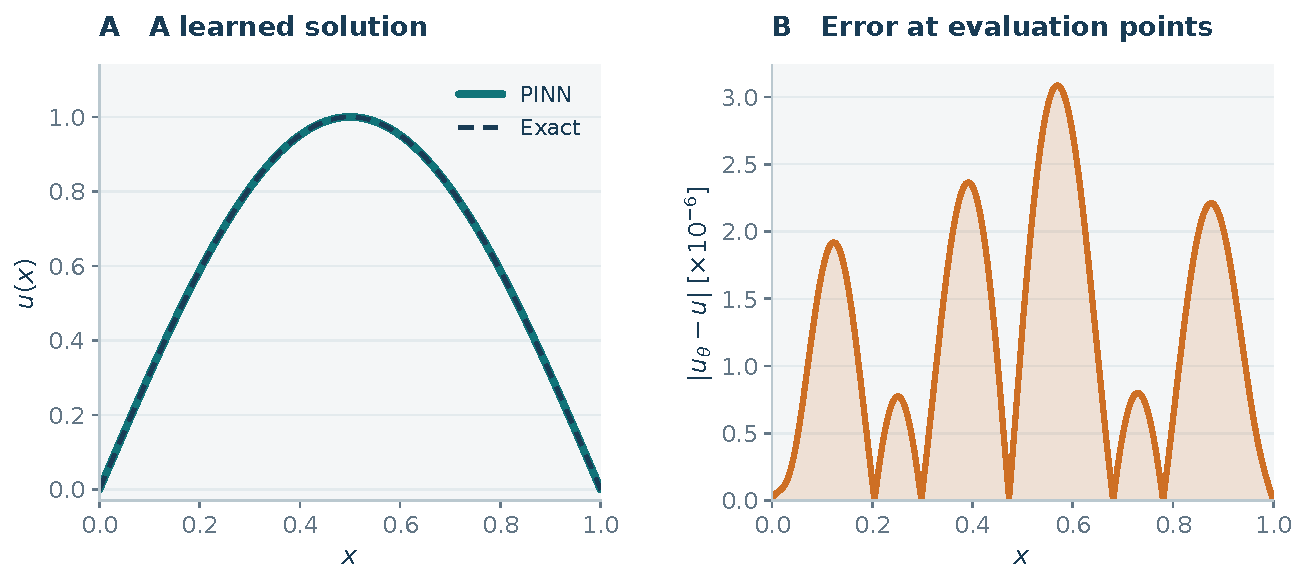
\includegraphics[width=\textwidth]{experiments/figures/poisson_1d.pdf}
\begin{block}{Measured on 1,001 evaluation points}
Relative $L^2$ error: \textbf{\ForwardLtwo}; maximum absolute error:
\textbf{\ForwardMaxError}. The endpoints are exactly zero by construction.
\end{block}
\labnote{The error panel resolves differences hidden by overlapping solution curves.
All reported errors are numerical grid estimates.}
\end{frame}

\renewcommand{\slideid}{L3-PY04}
\begin{frame}[c]{Python lab 2: the same idea in two dimensions}
\small
\[
 -\Delta u=2\pi^2\sin(\pi x)\sin(\pi y),\qquad
 u|_{\partial(0,1)^2}=0.
\]
\lstinputlisting[style=pythonlab]{experiments/snippets/poisson_2d_loss.py}
\end{frame}

\renewcommand{\slideid}{L3-PY05}
\begin{frame}[c]{Python output: a field, a reference, an error map}
\small
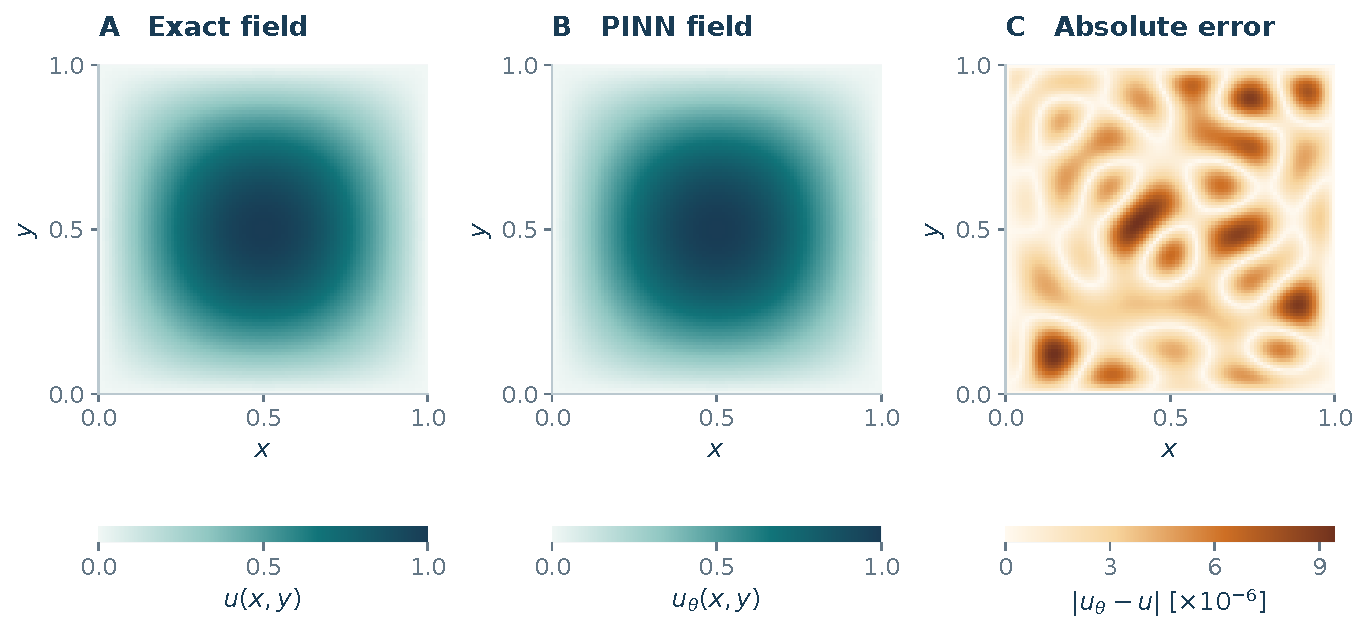
\includegraphics[width=\textwidth]{experiments/figures/poisson_2d.pdf}
\begin{block}{Validate on a separate $101\times101$ mesh}
Relative $L^2$ error: \textbf{\TwoDLtwo}; maximum absolute error:
\textbf{\TwoDMaxError}.
\end{block}
\labnote{Exact and learned fields share one color scale. The error uses its own
scale to reveal where the approximation is least accurate.}
\end{frame}
\renewcommand{\slideid}{L3}
